\documentclass[preprint]{acm_proc_article-sp}
%\documentclass[preprint]{sig-alternate}
\usepackage{url}
\usepackage{graphicx,subfigure}
\usepackage{xspace}
\usepackage{multirow}
\usepackage{amsmath}
\usepackage[hang,small,bf]{caption}
\DeclareCaptionType{copyrightbox}

\DeclareMathOperator{\Argmax}{argmax}
\newcommand{\PosC}{\mathrm{Spam}}
\newcommand{\NegC}{\mathrm{Ham}}
\newcommand{\ie}{{\em i.e.,}~}
\newcommand{\eg}{{\em e.g.,}~}

\renewcommand{\normalsize}{\fontsize{10.5pt}{12.5pt}\selectfont}

\setcounter{page}{1}
\pagenumbering{arabic}

\newenvironment{denseitemize}{
\begin{itemize}[topsep=2pt, partopsep=0pt, leftmargin=1.5em]
  \setlength{\itemsep}{4pt}
  \setlength{\parskip}{0pt}
  \setlength{\parsep}{0pt}
}{\end{itemize}}

\newcommand{\eat}[1]{}

\begin{document}

\title{Feature Selection and Classification of \\
    Spam on Social Networking Sites}

\numberofauthors{3}
\author{
Antonio Lupher,
Cliff Engle,
Reynold Xin\\\\
\texttt{\{alupher, cengle, rxin\}@cs.berkeley.edu}
}

\maketitle
\begin{abstract}
Social networking sites (SNSs) see a variety of spam and scams targeted at 
their users. In contrast to the limited amounts of information available beyond 
message text and headers when analyzing email spam, spam on SNSs is often accompanied 
by a wealth of data on the sender, which can be used to build more accurate detection mechanisms. 
We analyze 4 million private messages as well as other public and private data from 
a popular social network in order to gain insight into the various features of 
spam messages and the accompanying user accounts data available to site operators. 
We use these insights to choose features that best differentiate spammers from 
legitimate, ``ham," users.  Finally, we extract these features from the site's data 
and use them to train and evaluate classifiers.
\end{abstract}

\maketitle

\section{Introduction}

Social networking sites (SNSs) of any significant size witness a constant flow of spam, 
scams and phishing attacks.  The nature of this unwanted activity, which we henceforth refer to 
collectively as ``spam" can be 
quite diverse, specific to a site's target audience and often not easily detectable. Marketers 
spam members with unwanted advertisements, fraudsters lure users with advance fee frauds and 
other confidence tricks, while others may attempt to steal user information by directing users 
to external phishing pages. 

Sites with global reach see communication among members in a variety foreign languages with 
varying levels of ability. This means that much benign content shares characteristics including 
misspellings, awkward phrases, and so on, that might have made certain types of common frauds and spam 
more easy to distinguish on US-based (or English-language) sites. Likewise, simple regional IP-based 
filtering to target high-spam countries like Nigeria and Ghana would prevent legitimate users 
located on blocked networks from accessing the site.

In contrast to email spam, social spam often has a more personal component, since both spammers 
and legitimate users (``ham" users) have accompanying profiles with descriptive information. This can 
lead to more drawn-out, conversational attempts by spammers to approach users, since communication 
is more immediate (in the sense that users may see that they are online at the same time, may 
visit each others' profiles, etc.). However, the additional user data inherent in SNSs also 
offers a bountiful supply of data that site operators can mine to detect spam more effectively.

Most research on social networking spam has been done at a distance, using data collected 
either through scraping or artificially attracting spammers through ``honeypot" accounts. This 
paper leverages access to private messages, metadata and account details from a popular SNS 
to study the characteristics of social spam as well as the features and classifiers that 
sites can use to detect it.

\subsection{Approach}

We examine in detail the classes of malicious and benign
content that users encounter on social networks. We do this by analyzing
data available from InterPals, an international social network
for cultural exchange and language practice. The site
attracts a wide variety of financial scams, ranging from Nigerian
``419" scams to romance scams. Another prevalent problem is spam with
links to third-party websites, directing users to various porn/webcam
sites, phishing sites or various untrustworthy online marketplaces.

We examine various methods of detecting and preventing abuse
on the site, including those measures that have already been taken
(\eg various heuristics including IP-based location anomaly detection,
frequency capping, duplicate account detection, etc.). We then analyze 
message and user account data to try to identify characteristics that 
best differentiate legitimate users from malicious ones. By mining this data, 
 we extract features to build and evaluate classifiers that can detect unwanted behavior 
programmatically. The large volume of data available to us, although we do 
not use all of it, provides a unique perspective both on the types of
malicious content that exist on such sites as well as on the
effectiveness of classifier-based approaches to identifying
these activities.

This paper investigate several machine learning techniques to 
detect spam in private messages. We train and evaluate Naive Bayes, 
linear regression, and support vector machine (SVM) 
classifiers. Our implementations used a variety of tools, 
including Matlab, ScalaNLP, LIBSVM, Lucene and Spark, 
an in-memory distributed computing framework designed for machine 
learning and iterative computation.

\subsection{Data sets}

We enjoyed unrestricted access to the data of InterPals.net, a SNS with 
over 1.3 million active members. The data from this site includes a corpus of over a 
100 million private messages and another 2 million messages that have been 
labeled as spam  and deleted by users. Other data includes 40 million or so ``wall" 
comments, 5 million photos and 8 million photo comments. 

\section{Related Work} 

The rapid growth of social media has made SNSs increasingly attractive targets 
for spam and fraud, leading to a proliferation of sophisticated attacks. This 
trend is reflected in recent research, as papers 
have focused on identifying and classifying the various types of social media spam. 
Many of these studies employ techniques previously used to combat conventional 
email and web spam. SNSs also provide opportunities to take advantage of user 
reputation and other social graph-dependent features to improve classification. 
Nevertheless, most research has been carried out on publicly-available data 
from SNSs, making it unfeasible up until now to measure the effect of private user 
data on algorithms for detecting site misuse.

\subsection{Social Spam Features}

Heymann et al. \cite{heymann} survey the field of spam on SNSs, identifying 
several common approaches. Identification-based approaches identify spam to 
train classifiers based on labels submitted by users or trusted moderators. 
Rank-based approaches demote visibility of questionable content, while interface-based 
approaches apply policies to prevent unwanted behavior. This work groups 
classification-based approaches with detection, although classifiers can be 
used in conjunction with user information to prevent spam before it happens.

A number of researchers have focused on collecting, identifying features 
and classifying various genres of spam on social networks. Zinman and 
Donath \cite{zinman} extract bundles of profile-based and comment-based 
features from MySpace profiles, but the relatively poor performance of their classifier highlights 
the difficulties in manual classification of social network spam. Several 
studies \cite{stringhini, lee} take the approach of baiting spammers with social ``honeypots", profiles 
created with the sole intent of attracting spam. They 
then use the data collected to train classifiers with features including 
friend request rate and ratios of URLs to text. Webb et al. \cite{webb} use 
the honeypot approach as well and provide examples of various types of spammers, 
the typical demographics of their profiles, as well as the web pages that they tend to advertise. 

Gao et al. \cite{gao} look at Facebook wall posts, analyzing temporal properties, 
URL characteristics, post ratios and other features of malicious accounts. They 
also pinpoint various spam ``campaigns" based on products advertised in a given 
time frame. They note that spam on Facebook often exhibits burstiness and is mainly 
sent from compromised accounts. Benevenuto et al. \cite{benevenuto} identify 
social attributes of spam and ham on video SNSs (in this case, they scraped data from 
YouTube), including video view counts, comment counts and user public profile attributes. 
They then use a support vector machine (SVM) for classification, yielding 96\% accuracy in detecting 
advertisers (``promoters"), but only accurately identifying 57\% of examples of more general spam.

Not all undesirable content on SNSs is necessarily spam or a scam. SNSs and 
online communities witness inappropriate user behavior, where users post offensive 
and harassing content. Yin et al. \cite{yin} combine sentiment analysis and profanity 
word lists with contextual features to identify harassment on datasets from Slashdot 
and MySpace. Other work looks at SNSs as platforms to collect data about users in 
order to aid direct attacks on the user's computers or to compromise a large 
number of accounts. \cite{patsakis, huber}

\subsection{Social Spam Detection Systems}

SocialSpamGuard \cite{jin} is a social media spam detection system that analyzes 
text and image features of social media posts. The demo system uses GAD 
clustering \cite{jingad} for sampling spam and ham posts, then trains a 
classifier with text and image features. However, the system is built on top 
of Facebook features that are publicly accessible and thus cannot make use of 
sensitive user data (\eg IP addresses) to increase its effectiveness. 

De Wang et al. \cite{wang} propose a cross-site spam detection framework to share 
spam data across all social networking sites, building classifiers to identify spam 
in profiles, messages and web pages. This multi-pronged approach lends itself to 
associative classification, in which, for example, a message would be classified as 
spam if it contains a link to a web page that has a high probability of being spam. 
Unfortunately, the differing characteristics of various social networks \eg the length 
of messages in Facebook vs. Twitter, can reduce the benefits of sharing spam corpora 
across diverse sites.

Facebook \cite{stein} provides an overview of their ``immune system" defenses 
against phishing, fraud and spam. The system is composed of classifier services, an 
ML-derived Feature Extraction Language (FXL), ``feature loops" or services that aggregate 
and prepare features for classification and a policy engine to take action on suspected misuse. While 
the discussion remains high-level and includes few implementation particulars, it does 
include significant detail on the various types and characteristics of undesirable 
activity on the site, including fake profiles, harassment, compromised accounts, malware 
and spam. 

In contrast to research that focuses on dynamically detecting spam based on user 
activity, Irani et al. \cite{irani} show that static features associated with user signups 
on MySpace are enough to train an effective social spam classifier. They note that
C4.5 decision tree algorithms provide better performance than Naive Bayes in this case. 
As in other works, this only examines publicly available profile information collected 
by social honeypots. Private data collected on users including browser features, IP addresses 
and geographic location would conceivably improve classifier performance substantially.

Bosma et al. \cite{bosma} explore user-generated spam reports as a tool for building an unsupervised 
spam detection framework for SNSs. Their approach counts the number of spam reports against a 
suspected spammer and adds weight to reports based on user reputation. Determining reputation 
and trustworthiness of users in social networks has been well studied \cite{bian, guha, zhang} 
and appears to be a promising addition to social spam classification. The framework uses a 
Bayesian classifier and links messages with similar content, but does not take into account 
other features. Nevertheless, this is one of the few studies to test its framework on 
non-public data, including private messages, spam reports and user profiles from a 
large Dutch social networking site.

\subsection{Email \& Web Spam}

Much work has been done on protecting traditional email systems from spam. 
Blanzieri \cite{blanzieri} offers a comprehensive overview of machine learning techniques 
that can be applied to email filtering. Hao et al. \cite{hao} describe a reputation 
engine based on lightweight features such as geographic distance between sender and 
receiver and diurnal patterns. While the target was conventional 
spam, monitoring sender reputation and using similar features (\eg time-of-day when messages 
were sent), seesm applicable to spam on SNSs as well.

Whittaker et al. \cite{whittaker} describe a scalable phishing machine learning 
classifier and blacklisting system with high accuracy. Since a considerable 
amount of social media spam includes links to phishing sites, being able to 
detect them is critical. Along similar lines, Monarch \cite{thomas} is a 
system that provides scalable real-time detection of URLs that point to spam web pages as 
determined by URL features, page content and hosting properties of the target domain.

Blog comment spam have also attracted considerable attention from researchers who 
have applied machine learning \cite{kolari, nag} techniques including SVMs and Bayesian classifiers.
Mishe et al.\cite{mishne} employ language modeling to find semantic discrepancies between 
the blogs on which link spam comments are posted and the target sites (which might, for example, 
contain adult content). Likewise, Markines et al. \cite{markines} apply similar techniques 
including SVMs and boosting (AdaBoost) to spam on social bookmarking sites.

\subsection{Machine Learning and Data Mining}

Many of the data mining algorithms used to detect spam and patterns of misuse 
on SNSs are designed with the assumption that the data and the classifier are 
independent. However, in the case of spam, fraud and other malicious content, 
users will often modify their behavior to evade detection, leading to degraded 
classifier performance and the need to re-train classifiers frequently. Several 
researchers tackle this adversarial problem. Dalvi et al. \cite{dalvi} offer a 
modified naive Bayes classifier to detect and reclassify data taking into account 
the optimal modification strategy that an adversary could choose, given full knowledge of 
the classifier model and parameters, but without the ability to tamper with the 
classifier's training data. The authors show that the optimized classifier's counter-strategy 
is substantially more effective than a standard classifers in the cases examined: 
adversaries adding words, adding length and substituting words with synonyms. 
Lowd and Meek \cite{lowd} provide a framework for reverse engineering a 
classifier to determine whether an adversary can efficiently learn enough 
about a classifier to effectively defeat it.

\section{Data Sets}

For this project, we had unlimited access to data from InterPals, a site for users who 
wish to communicate with people from other countries, whether for language practice, cultural 
exchange or friendship. Users sign up by completing a registration form with 
information about themselves, including age, sex and location. After registering, users 
can expand their profile page to include self-descriptions, interests, languages they speak,  
photographs, etc. After clicking on an activation link sent to their email address, a user can 
begin to interact with others on the site via private message, public ``wall" posts, comments 
on photos and on a bulletin board system.

\subsection{Current Anti-Spam Measures}

Currently, the site combats spam and other Terms of Service violations 
through volunteer moderators. Users can report content, including private messages, 
profiles and photographs, to moderators by using a form that includes a drop-down menu of 
pre-selected reasons with the option to add a more detailed message in a text field. 
Likewise, the message interface allows a user to report a private message as spam with a single 
click. Moderators have access to a queue of these reports. In addition to the material 
being reported, moderators are able to make decisions based on the data from the reported 
user's account, including outgoing private messages, IP addresses, as well as a list of 
other users who have logged in from the same computer (determined via IP address, cookies, as well 
as by rudimentary browser fingerprints). Moderators can then decide to delete the user, send a warning, 
or clear reports on a user. All moderator actions require them to annotate their decision with a 
brief log message. When deleting a user, moderators have the option of flagging the 
reported message (if there is one) as spam or of flagging all of the user's outgoing private messages 
as spam.

Other anti-spam measures include widespread use of CAPTCHAs across the site and 
frequency caps on activities that involve contact with other users. Short-window 
frequency caps are in place for all users, limiting the 
number of messages that can be sent per short time interval (1, 5 and 10 minutes). New users 
are also subject to a per-day cap on the number of unique users with whom they are able to initiate 
contact. 

%- Users are able to filter messages by age, sex, continent and country. At this time, 
%- Duplicate account detection

\subsection{Spam Data Set}

At the beginning of this research project, slightly over two million messages had 
been flagged by moderators as spam. We extracted the contents of exactly 2 million 
spam-labeled messages from accounts deleted by moderators between October 2011 
and March 2012. As moderators can flag a user's entire list of outgoing messages 
as spam on deletion, the earliest sent dates of some messages in our data set begin in 
May 2010. 

InterPals stores private messages and user account data in a number of separate MySQL tables. 
Account information for deleted users is stored for six months, so account details for all spam 
and ham accounts were available. Extracting the data of interest to this project required 
dumping the contents from a query with multiple joins and aggregations across 8 tables with a 
combined size of 154 GB. To minimize the impact on the load of the site's production database 
instances, we took an LVM snapshot of a replication instance (the production database has one master and one 
slave) and cloned the database to a spare server. 
In addition to using SQL to extract the data, we wrote Perl scripts to clean the data, tokenize 
messages and prepare data for further processing. The methodology section offers more details 
on precisely which items of data were collected and why.

\subsection{Ham Data Set}

Unlike spam messages, we did not have access to a comparable corpus of human-labeled ham 
messages. To simplify the labeling of ham messages, we made the assumption that messages remaining in 
the inboxes of active users after a period of several months would most likely not be spam. 
Consequently, we extracted a working set of 2 million ham messages that were sent in late December 2011 and early 
January 2012 and still existed in the recipient's inbox as of March 2012. To reduce the 
possibility of collecting messages sent by uncaught spammers to inactive or dormant users, 
we selected messages only from senders and to recipients who had logged in within the last two 
weeks. As in the case of the spam data set, we collected two million messages with associated account 
data and merged them into text files for feature extraction.

\subsection{Categories of Spam}

In the course of collecting the data, we observed a number of distinct classes of 
undesirable messages. Our ongoing observation of spam on the InterPals website provided 
direct intuition into the major classes of unwanted behavior that we classified as spam for 
this project. We noted the following broad categories:

\begin{itemize}
\item \textbf{Advance fee fraud}, including inheritance, lotter, visa and customs-clearance scams
\item \textbf{Romance scams}, including ``mail-order bride" and military scams
\item \textbf{Sexual solicitation}
\item \textbf{Ads for porn sites}, primarily adult webcam and live chat sites.
\item \textbf{Ads for miscellaneous external sites}, often other SNSs
\item \textbf{Money muling}, often in the guise of high-paying ``stay-at-home" jobs or ``mystery" shopping
\item \textbf{Begging \& gift requests}
\item \textbf{Business proposals}
\end{itemize}

These categorizations are based only on cursory manual observation of a sample of several tens of thousands 
spam-labeled messages. We plan to quantify the volume of messages in each of these categories and 
attempt to provide a finer granularity of categorization (and more detailed level of description) in 
future research. 

%Analyzing the relevant terms in log comments entered by moderators when 
%deleting spammer accounts provides the following breakdown:

\section{Methodology}

We chose to focus on spam in private messages for this paper, given that messages account for 
a majority of user spam reports on the site. In addition to using the bag-of-words representation of 
the message content, we aimed to identify a subset of relevant ``expert" features 
based on public and non-public message and account information that would augment the classifier's 
accuracy. We first extracted a number of fields that we expected might improve classification. 

To choose a sample of relevant features, we computed statistics and generated histograms on 
the extracted features, comparing the ham and spam corpora. These statistics were generated 
using SQL on a table created from the merged and cleaned data generated in the process described 
above. We then chose a subset of these features to use for training and evaluating our classifiers.

\subsection{Message Features}

\textbf{Message body \& subject:} We extracted both the message body and subject from 
each spam and ham message. The cleaning script generated two additional features based 
on this. First, we counted the frequency of non-standard punctuation (we noticed that many 
spam messages would, for example, put spaces before commas, periods and quotation marks, 
while omitting spaces after these characters). Second, we calculated the ratio of uppercase to 
lowercase letters in the text, after observing relatively high amounts of uppercase text in 
spam messages.
%% add numbers

\textbf{Recipient age, sex and country:} These fields were the age, sex and ISO 3166-1 alpha-2 code of the message 
recipient, as listed on their profile. Unfortunately, due to data collection issues, this data was only available 
for the most recent 11,000 spam messages. While the male-to-female ratio of the recipients was very close to that 
of non-spam recipients (both were 47\% male to 53\% female), we found that the age of recipients was typically higher.

\textbf{Recipient replied:} This boolean value indicates whether the recipient replied to the message. We saw 
that the mean reply rate for ham messages was 81.77\% (SD: 38.61), while it was only 0.81\% (SD: 8.97) for spam messages. 

\subsection{Sender Account Features}

We chose message and user account features to analyze primarily by the amount of data that 
we had for each them, while making sure to include the most vital account information. 
Table \ref{tab:feats} offers statistics on a number of the account features that we examined. 

\begin{table}
\small
\begin{tabular}{|l|l|r|r|r|}
    \hline
    \textbf{Feature} & \textbf{Label} & \textbf{Mean} & \textbf{Median} & \textbf{Std. Dev.}\\
    \hline
    \multirow{2}{*}{Unique IPs} & Spam & 11.82 & 2 & 52.52\\
    & Ham & 175.51 & 64 & 322.19\\
    \hline
    \multirow{2}{*}{Sender Age} & Spam & 33.52 & 31 & 11.09\\
    & Ham & 24.86 & 22 & 10.30\\
    \hline
    \multirow{2}{*}{Photos} & Spam & 2.09 & 1 & 8.04\\
    & Ham & 15.69 & 6 & 43.40\\
    \hline
    \multirow{2}{*}{Photo Albums} & Spam & 0.91 & 1 & 0.56\\
    & Ham & 1.89 & 1 & 2.43\\
    \hline
    \multirow{2}{*}{Friends} & Spam & 11.82 & 0 & 52.52\\
    & Ham & 23.26 & 10 & 58.91\\
    \hline
    \multirow{2}{*}{Recipient Age} & Spam & 39.98 & 41 & 12.69\\
    & Ham & 25.02 & 22 & 10.70\\
    \hline
    \multirow{2}{*}{Birth Day} & Spam & 12.31 & 10 & 8.52\\
    & Ham & 15.01 & 15 & 8.92\\
    \hline
    \multirow{2}{*}{Birth Month} & Spam & 5.85 & 5 & 3.33\\
    & Ham & 6.38 & 6 & 3.48\\
    \hline
    \multirow{2}{*}{Profile Desc. Len.} & Spam & 267.30 & 87 & 483.19\\
    & Ham & 439.33 & 267 & 613.26\\
    \hline
    \multirow{2}{*}{Fields Complete} & Spam & 22.15\% & 14.00\% & 30.75\\
    & Ham & 79.29\% & 86.00\% & 32.85\\
    \hline
    \multirow{2}{*}{Account Lifetime} & Spam & 900.36 h & 1.12 h & 4163.25\\
    & Ham & 8963.19 h & 5297.09 h & 11750.39 \\
    \hline
\end{tabular}
\caption{Feature statistics}
\label{tab:feats}
\end{table}

\textbf{Sender Country:} The distribution of countries as stated by users on their profile and as 
revealed by their IP address differed remarkably between the spam and ham user groups. 
48\% of spam users claimed to be from the United States, with the next most popular 
countries being the UK, Ghana, Senegal, Germany and Canada taking combined 25\%. 
In contrast, only 15\% ham users claimed to be from the United States, with Russia, 
Korea, UK, France and Germany combining for 24\%. This distribution of profile countries can 
be seen in Figure \ref{fig:cprof}.

\begin{figure}[h]
    \centering
    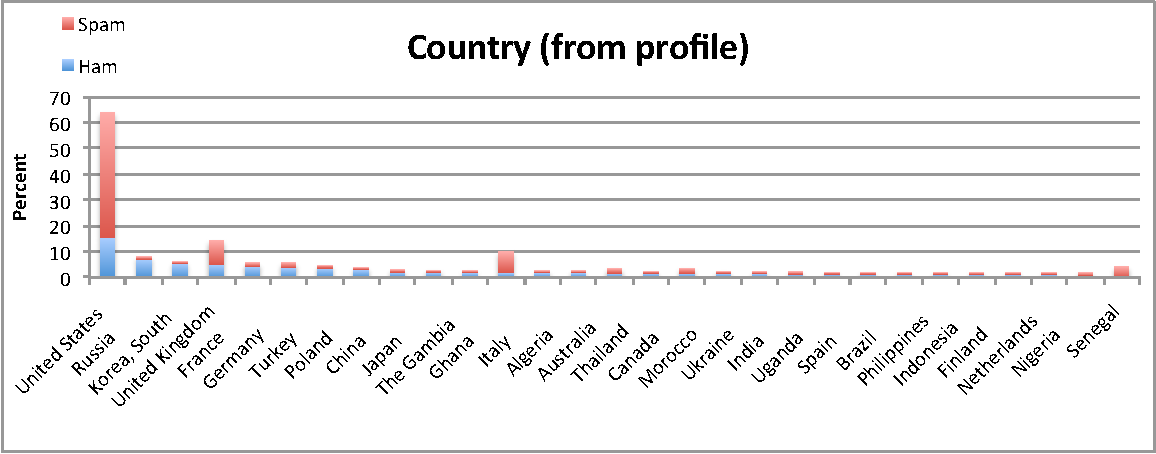
\includegraphics[width=\linewidth]{figures/country-prof.pdf}
    \caption{Country as stated on user profile}
    \label{fig:cprof}
\end{figure}

Users are free to choose any country on their profile. We record each IP address from which a 
user logs in to the site. By examining the distribution of countries (using the MaxMind GeoIP
database\cite{maxmind}) associated with the unique IP addresses (Figure \ref{fig:cip}), we see that the top 
countries for spammers are significantly different, while the top ham countries are 
virtually unchanged. Furthermore, only 30\% of the IP addresses of spam users who 
claimed to be from the United States actually mapped back to a US-based ISP, with a combined 
46\% indicating a Ghana, Nigeria and Senegal ISP (Figure \ref{fig:usaspam}). This contrasts 
with the 73\% that US-based IP addresses comprised for ham users whose profiles stated that 
they were in the United States (Figure \ref{fig:usaham}). During feature extraction, we also 
generated a boolean feature (IP mismatch) indicating whether the IP-detected country and 
the profile country matched. 

\begin{figure}[h]
    \centering
    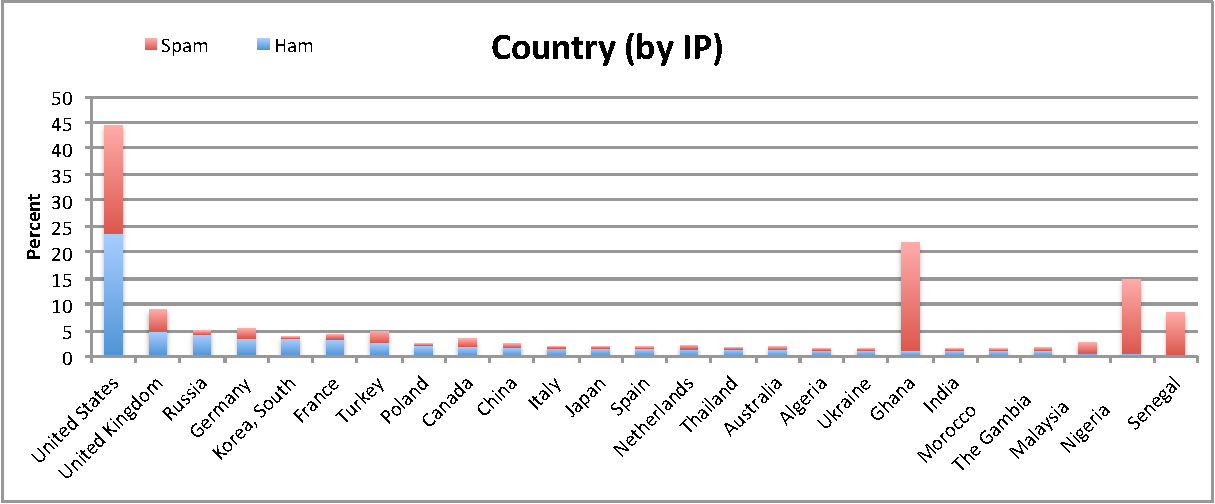
\includegraphics[width=\linewidth]{figures/country-ip.pdf}
    \caption{Country detected by IP address using MaxMind GeoIP database}
    \label{fig:cip}
\end{figure}

\begin{figure}[h]
    \centering
    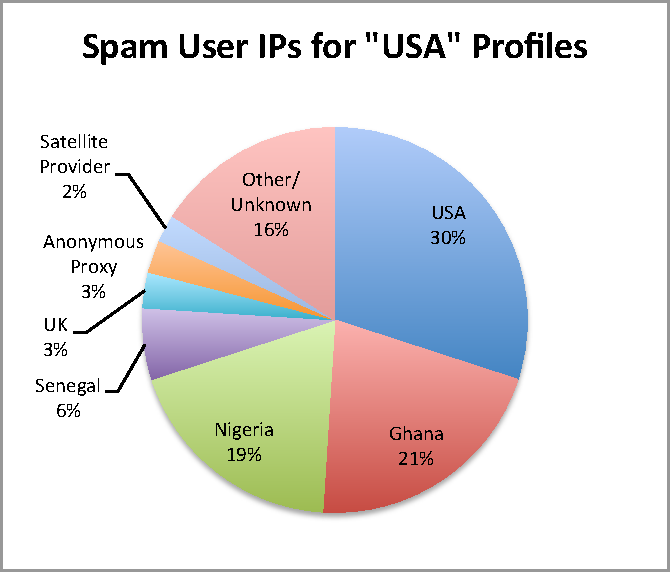
\includegraphics[width=\linewidth]{figures/ips-usa-spam.pdf}
    \caption{Distribution of IPs by country for spammers with profiles stating a USA location}
    \label{fig:usaspam}
\end{figure}

\begin{figure}[h]
    \centering
    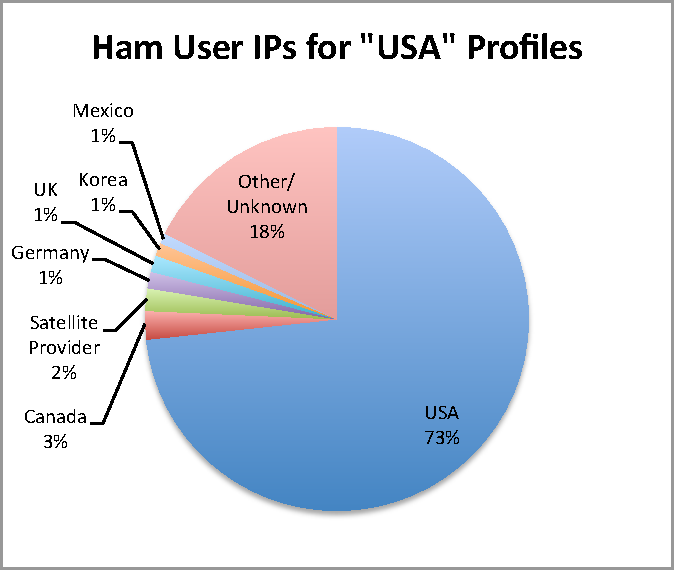
\includegraphics[width=\linewidth]{figures/ips-usa-ham.pdf}
    \caption{Distribution of IPs by country for ham users with profiles stating a USA location}
    \label{fig:usaham}
\end{figure}

\textbf{Sender IPs:} Spammers in general had a smaller number of unique IP addresses associated 
with them than ham users, as per figure \ref{fig:uniqip}. The median number of IP addresses for 
spam users was 2, whereas ham users saw a median of 64. This is likely due to the comparatively 
shorter length of time that spammers remain on the site before being deleted by moderators (Figure 
\label{fig:lifetime} show a histogram of the time elapsed between registration and message sending 
time).  Similarly, we believe that many legitimate users are behind NATs, yielding a high number 
of dynamic IP addresses. One possibility for future research is to investigate the ratio of 
unique IPs for users as a function of the time they have been registered. Likewise, examining 
unique /16 network blocks instead of unique IP addresses could mitigate the influence of NATs.

\begin{figure}[h]
    \centering
    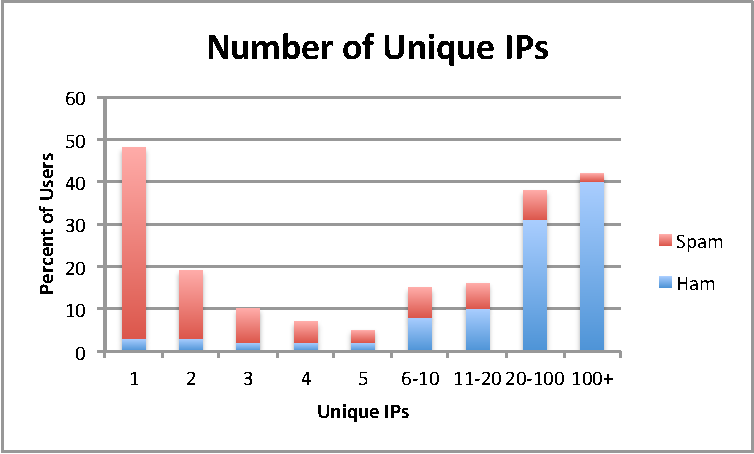
\includegraphics[width=\linewidth]{figures/unique-ips.pdf}
    \caption{Number of unique IP addresses associated with user account}
    \label{fig:uniqip}
\end{figure}

\begin{figure}[h]
    \centering
    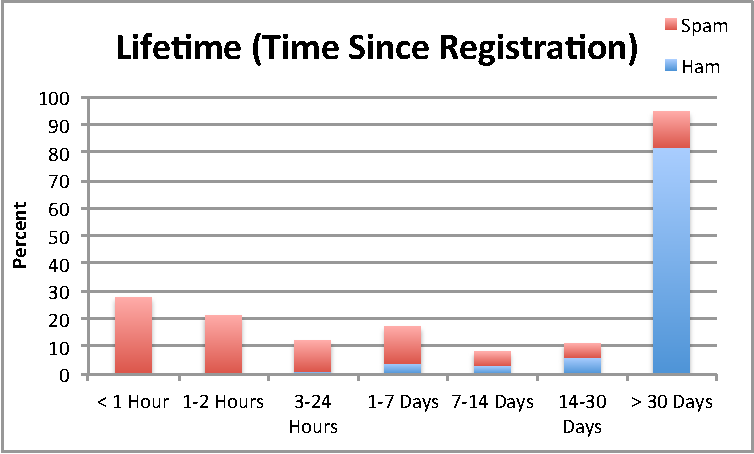
\includegraphics[width=\linewidth]{figures/lifetime.pdf}
    \caption{Sender account lifetime at the time that the message was sent}
    \label{fig:lifetime}
\end{figure}

\textbf{Sender Email:} Users must provide email addresses upon signup. The site does not allow users to contact other 
members before verifying that the email address provided is valid, via an account activation link sent to the signup 
address. Subsequent changes to a user's email address on file require a similar confirmation process. Thus, we can be certain 
that the email accounts that we extracted were in use by the senders, at least at the time of registration. 

\begin{figure}[h]
    \centering
    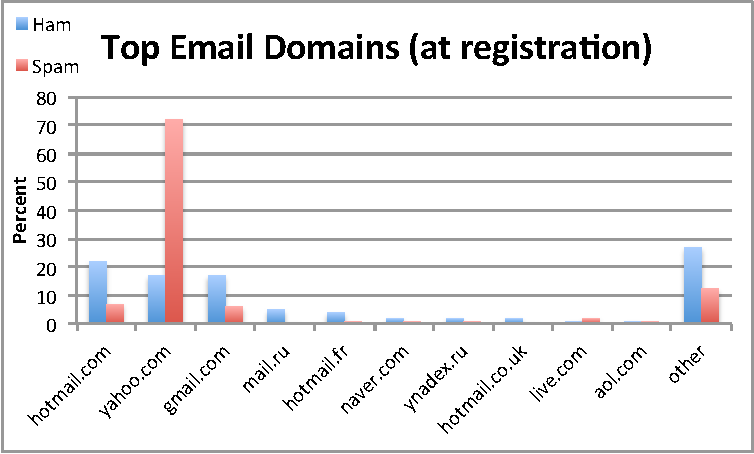
\includegraphics[width=\linewidth]{figures/email.pdf}
    \caption{Domain name of email provided at signup}
    \label{fig:email}
\end{figure}

In the data processing step, we extracted the domain name from each email address. We found that ham user email domains 
were distributed across top email providers in similar proportions (Hotmail, Yahoo and Gmail accounted for 22\%, 17\% and 17\% 
respectively). For spam user accounts, Hotmail, Yahoo and Gmail accounted for 7\%, 72\% and 6\% respectively. This striking 
predominance of Yahoo email accounts among spammers can be seen in Figure \ref{fig:email}. While we have no certain 
explanation for this, Figure \ref{fig:yspam} shows that Ghana and Nigeria alone account for 38\% of the IP 
addresses associated with these Yahoo accounts. This popularity of Yahoo among West African users has 
been noted before\cite{burrell} and appears to be due to the early penetration of Yahoo services in the region.

\begin{figure}[h]
    \centering
    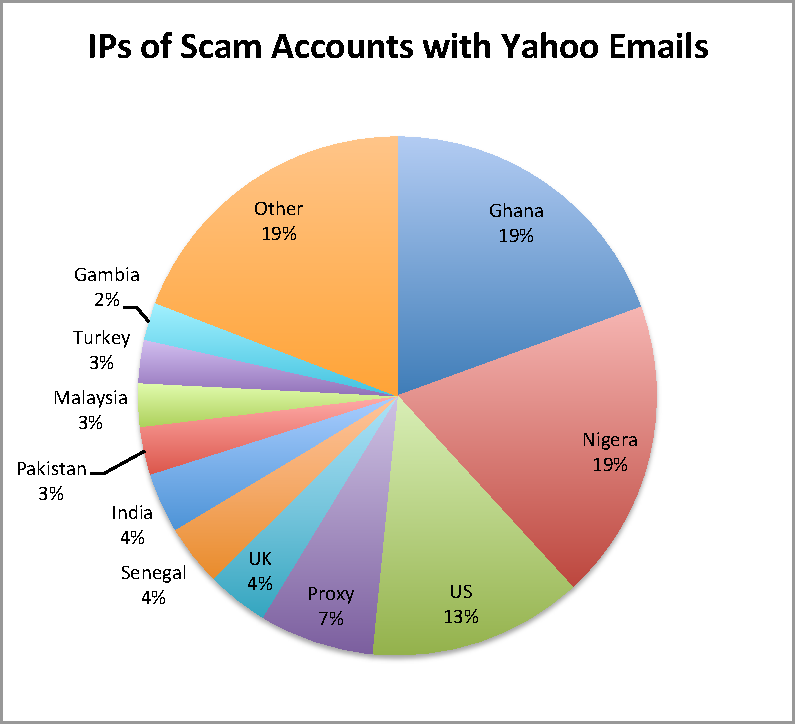
\includegraphics[width=\linewidth]{figures/yahoo-spam.pdf}
    \caption{IP distribution for scam accounts with Yahoo email addresses}
    \label{fig:yspam}
\end{figure}

\textbf{Sender \& Recipient Age:} The age indicated on their profile tended be higher for spam user than 
for ham users, with median ages of 31 and 22 respectively (Figure \ref{fig:sendage}). Likewise, the 
age of message recipients was higher for spam recipients that for recipients of ham messages, with 
median ages of 41 and 22 (Figure \ref{fig:recipage}). The sample size for spam recipient age 
was only 11,000 messages due to late data collection. We posit that the higher ages indicated on spam profiles, 
mirrored in recipient ages, reflects targeting of older users who are more likely to be financially 
stable. 

\begin{figure}[h]
    \centering
    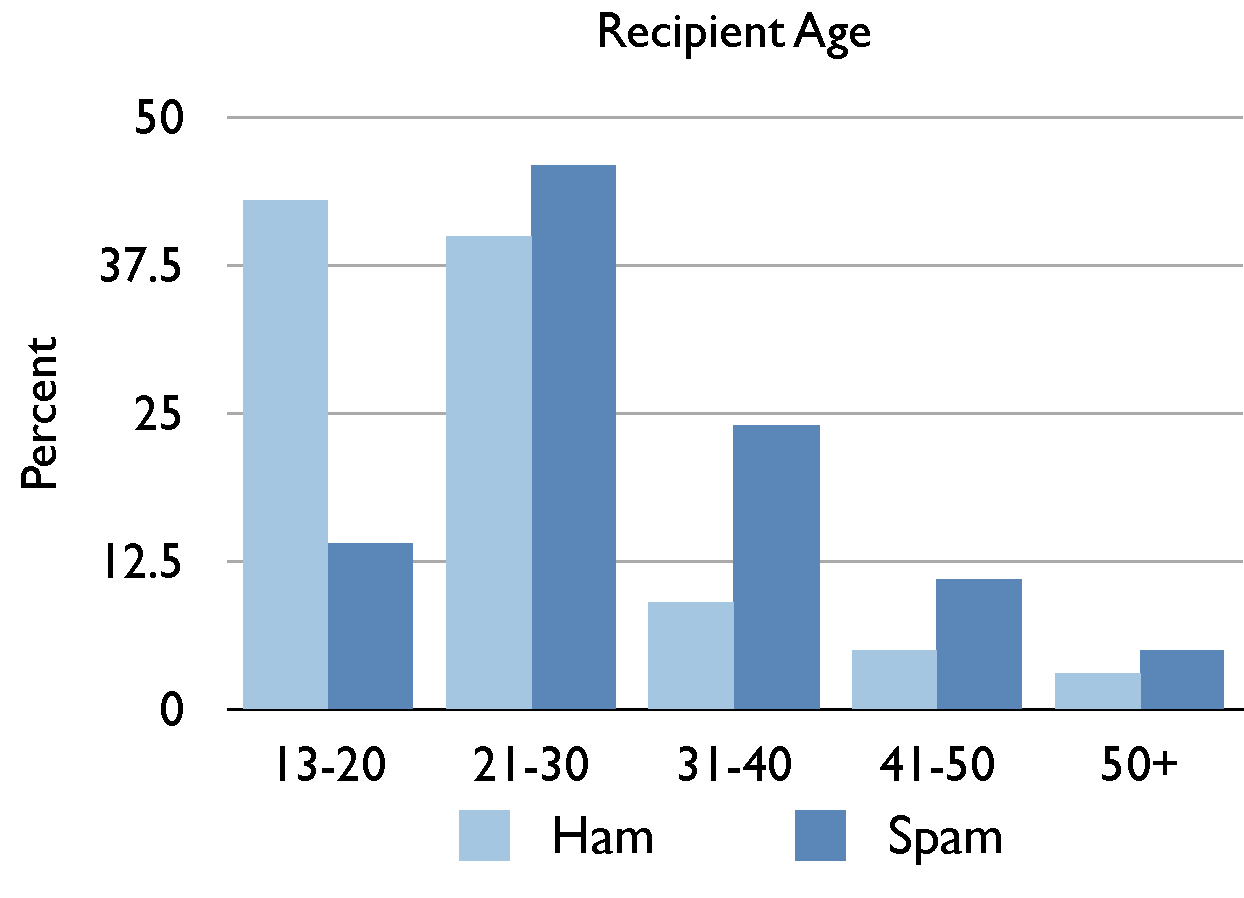
\includegraphics[width=\linewidth]{figures/recip-age.pdf}
    \caption{Age of message recipient as stated on user profile (Note that 2 million message spam sample 
        had only 11,000 messages with this information)}
    \label{fig:recipage}
\end{figure}

\begin{figure}[h]
    \centering
    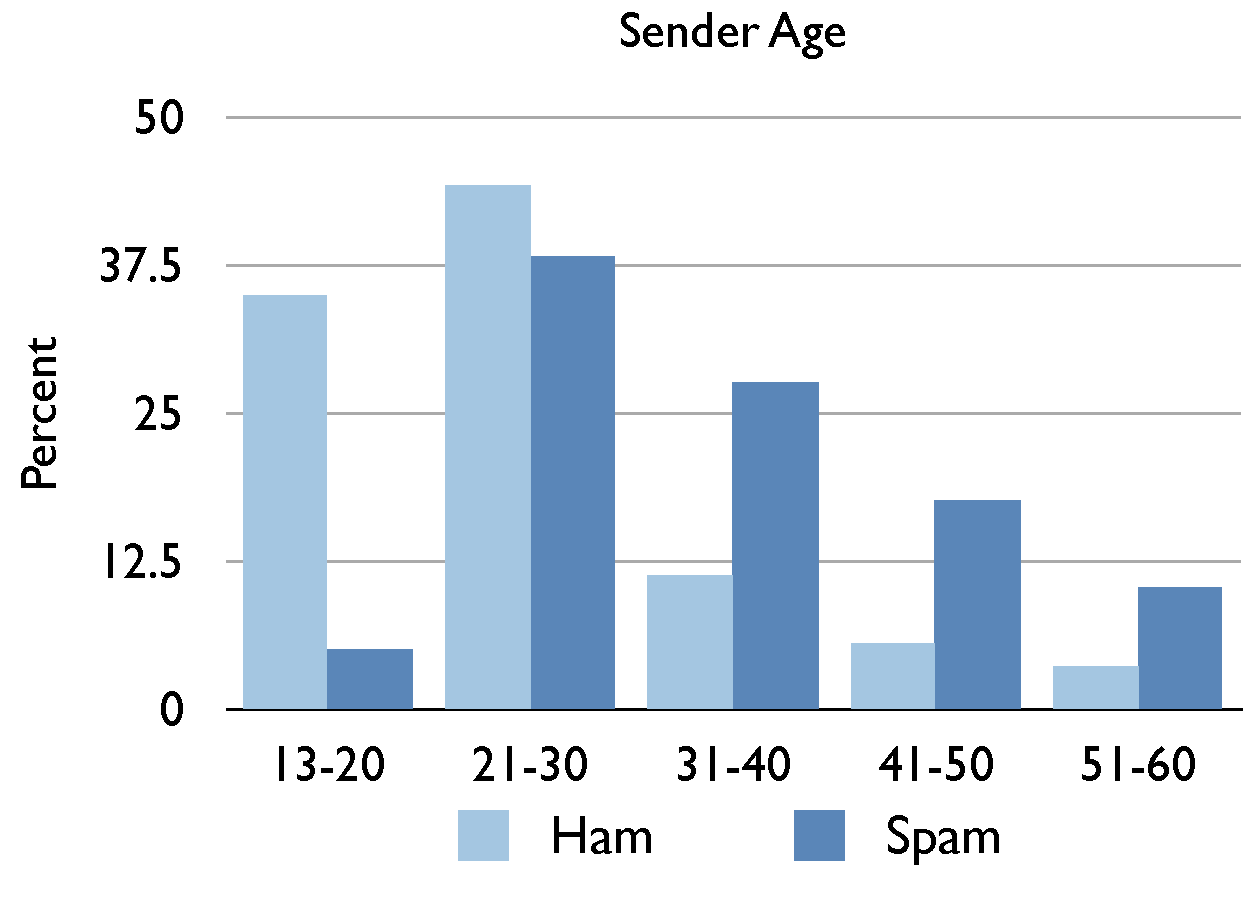
\includegraphics[width=\linewidth]{figures/sender-age.pdf}
    \caption{Age of message sender as stated on user profile. }
    \label{fig:sendage}
\end{figure}

\textbf{Sender Birthday:} We analyzed the birthdays and birth months of ham and spam users and noticed that spam users 
were more likely to have birthdays early in the month, and birth months early in the year. This is illustrated in 
Figures \ref{fig:day} and \ref{fig:month}. Given the drop-down select menus on the web site's registration form, reproduced 
Figure \ref{fig:drop}, it seems likely that this is due to an unwillingness on the part of spam users to 
scroll down to lower options (as well as, perhaps, a hesitance to disclose real birth dates). A similar trend is 
observed in the countries with the most discrepancies between IP-detected countries and countries stated on spam 
user profiles, with Afghanistan and Albania comprising 19\%, despite their relatively low representation on the 
site. 

\begin{figure}[h]
    \centering
    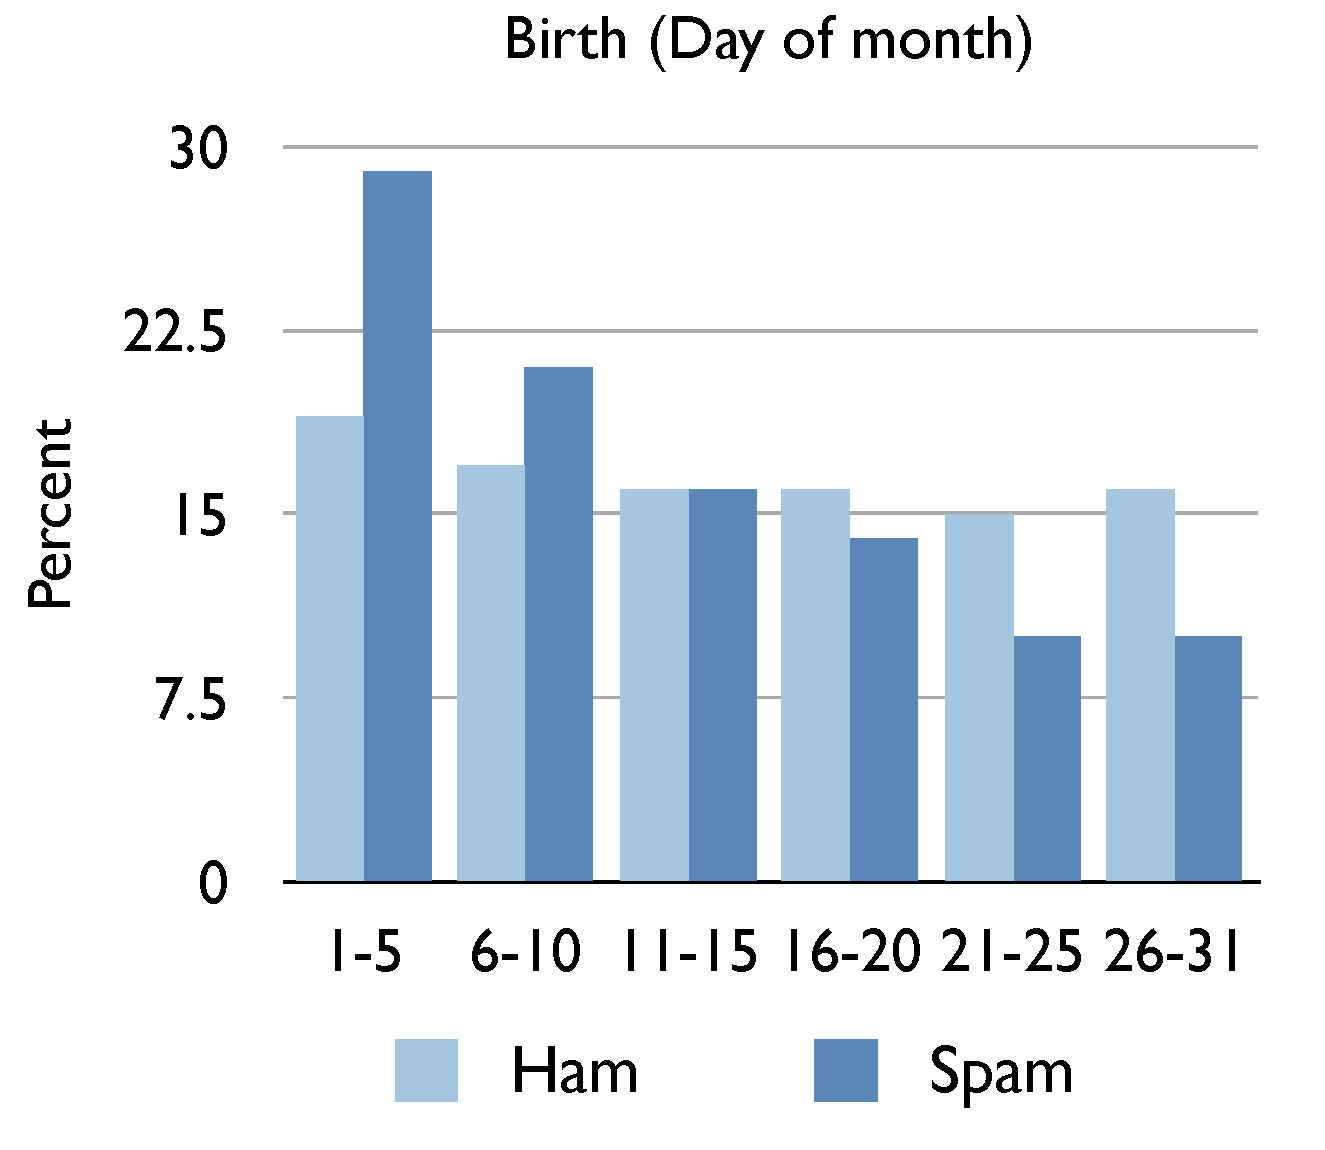
\includegraphics[width=\linewidth]{figures/dob-day.pdf}
    \caption{Date of month from birthday submitted by user at signup}
    \label{fig:day}
\end{figure}

\begin{figure}[h]
    \centering
    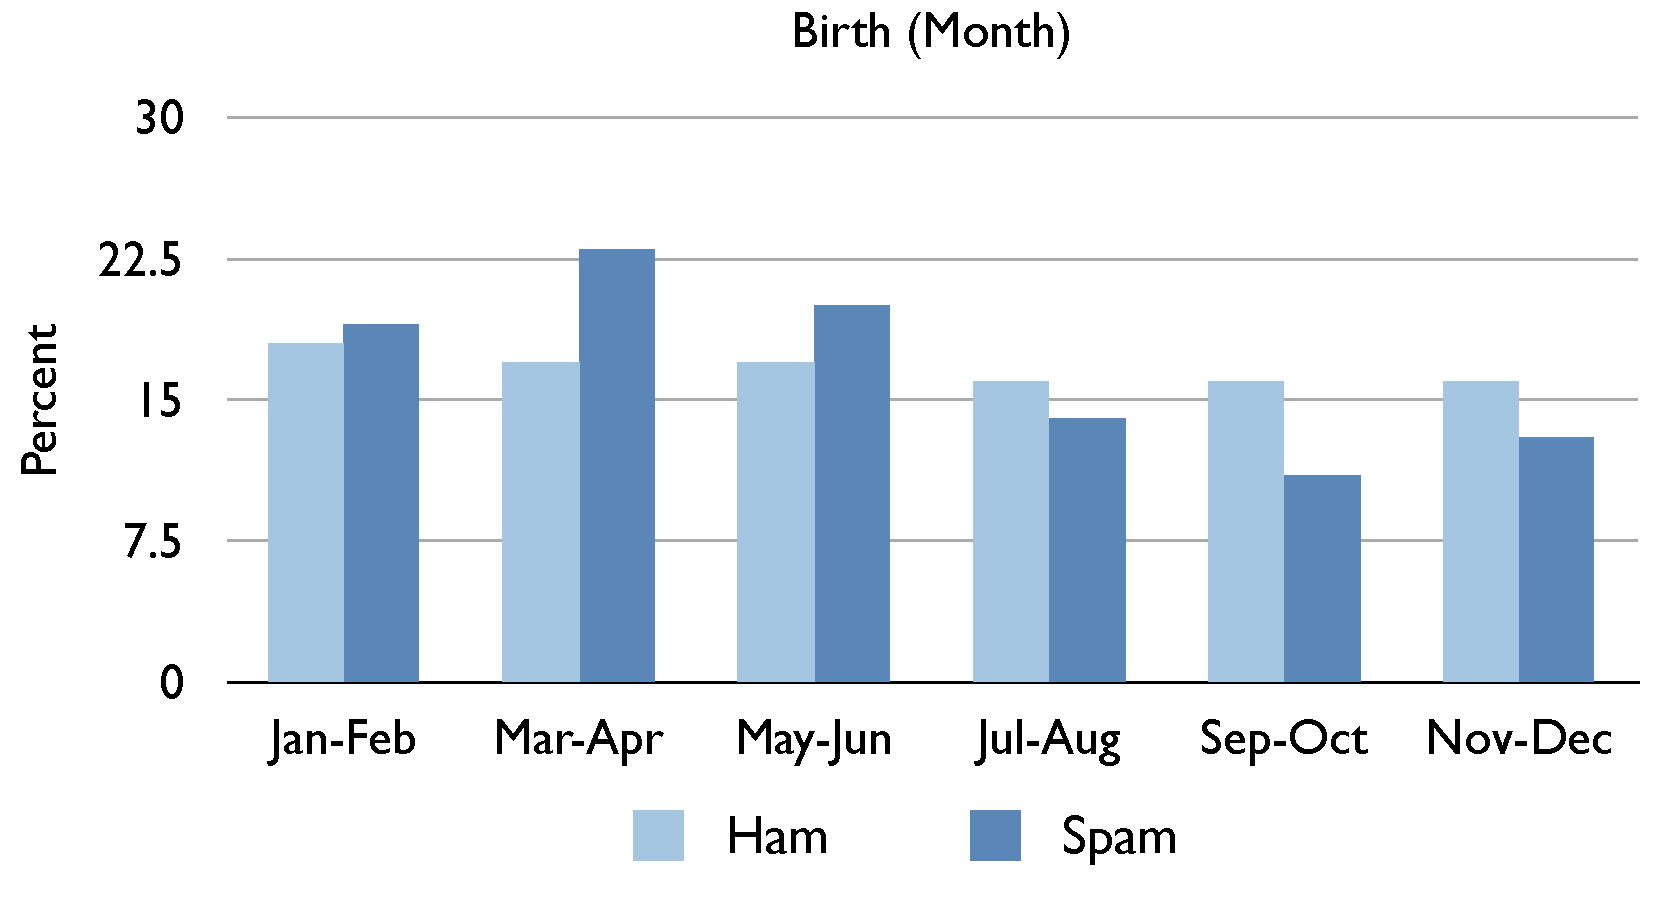
\includegraphics[width=\linewidth]{figures/dob-month.pdf}
    \caption{Month of birthday as submitted by user at signup}
    \label{fig:month}
\end{figure}

\begin{figure}[h]
    \centering
    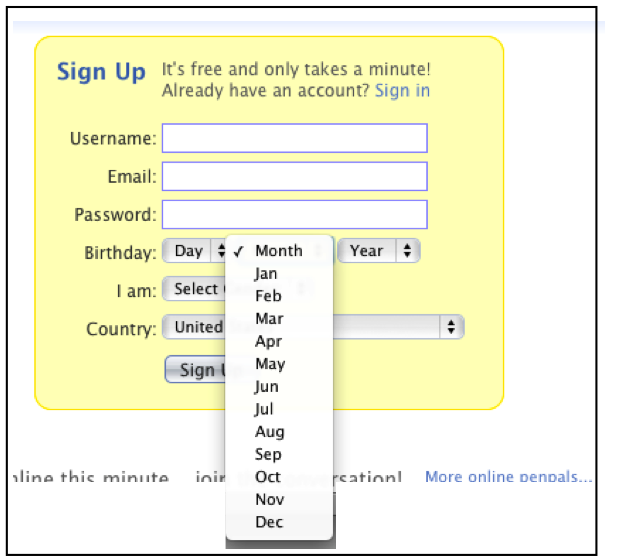
\includegraphics[width=\linewidth]{figures/dropdown.png}
    \caption{Drop-down select menu on signup form}
    \label{fig:drop}
\end{figure}

\textbf{Photos \& Friends:} We found that both the number of ``friends" that a user has (connections 
to other users) as well as the number of photos that user has uploaded were also indicative of their 
spam or ham reputation. Spammers typically had one or no photos, while ham users typically had larger 
quantities of both, as visible in Figures \ref{fig:photos} and \ref{fig:friends}. It is important to note, 
however, that we would expect a legitimate user's average number of photos and friends to grow over 
as a function of account lifetime. It would be quite reasonable for new ham users to have very photos 
or friends and we plan to further examine the relationship of these attributes over account lifetimes 
for both ham and spam users.

\begin{figure}[h]
    \centering
    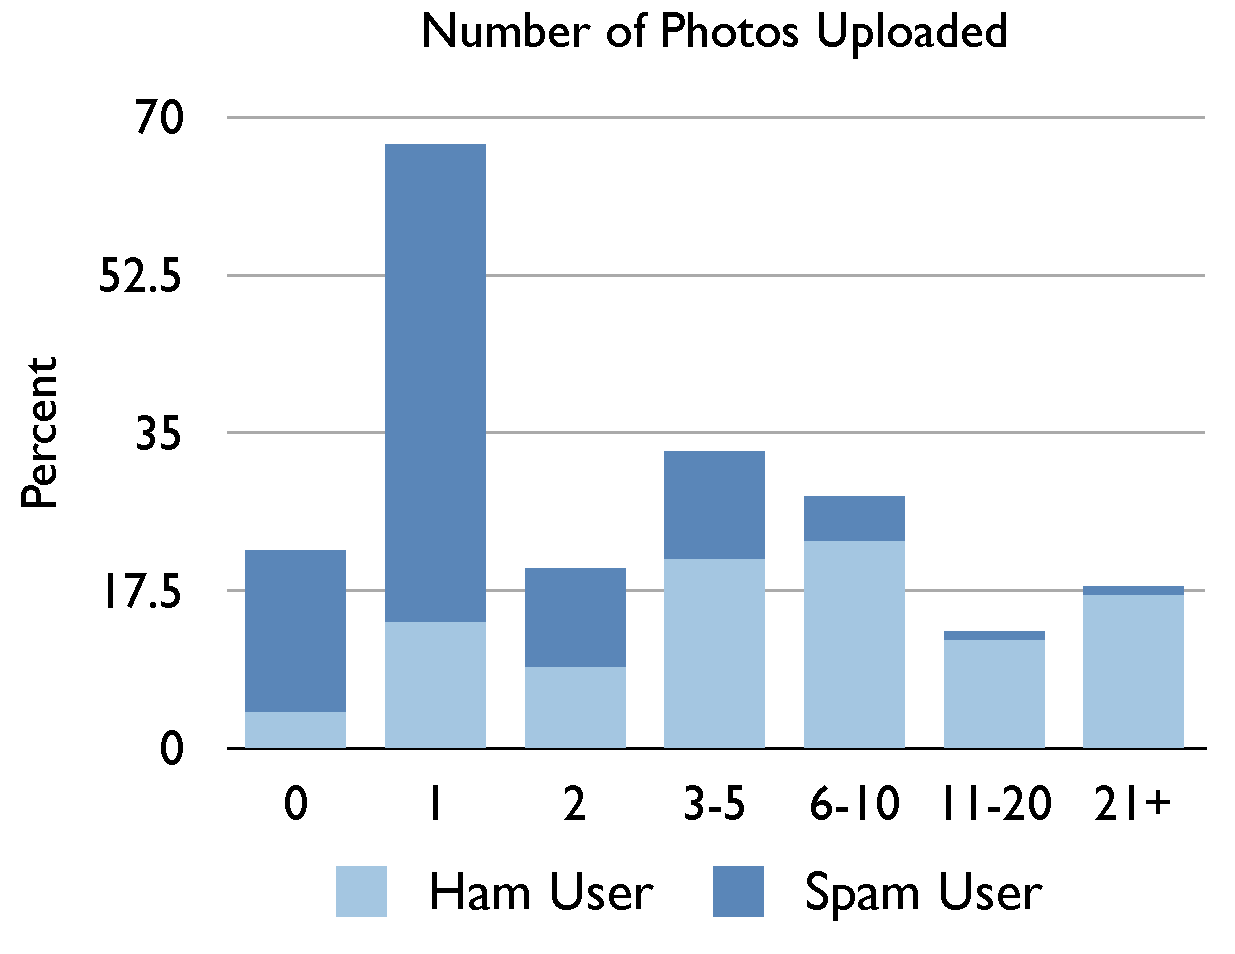
\includegraphics[width=\linewidth]{figures/photos.pdf}
    \caption{Number of photos associated with sender account}
    \label{fig:photos}
\end{figure}

\begin{figure}[h]
    \centering
    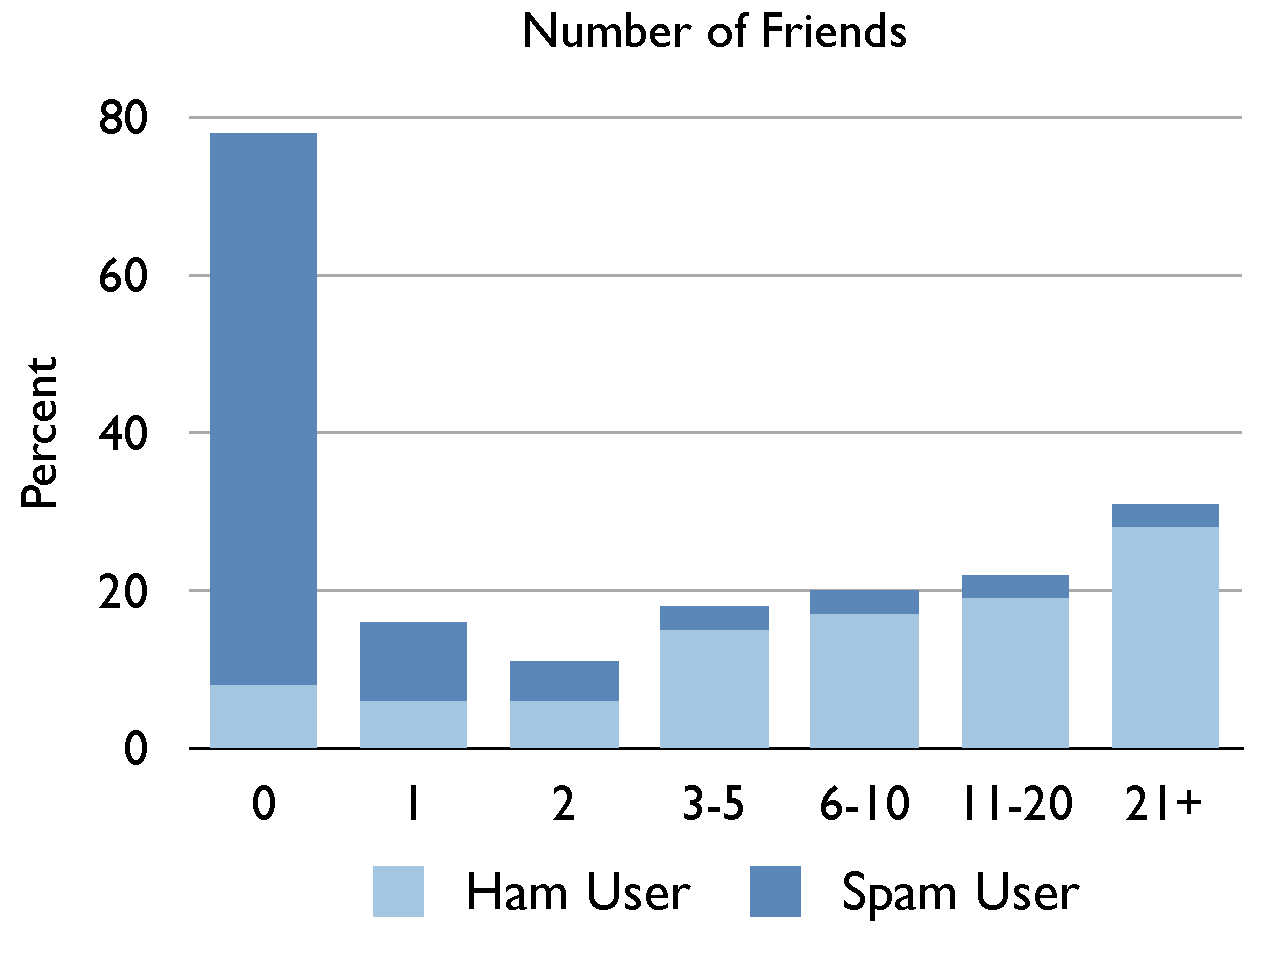
\includegraphics[width=\linewidth]{figures/friends.pdf}
    \caption{Number of friends associated with sender account}
    \label{fig:friends}
\end{figure}

\textbf{Username, Name:} While we collected these fields, we did not analyze them further, due to 
time constraints. Nevertheless, we saw considerable repetition in the usernames of scammers 
and it seems that analyzing the substrings in these fields could yield useful features.

\section{Classifiers \& Results}

Our goal in classification was not only to build an effective classifier for spam detection, 
but also to see how the presence of ``expert features", or features based on account and 
message metadata, could affect classifier accuracy. To this end, with of each of the classifiers 
we chose to implement, we evaluated performance on a bag-of-words representation of message data 
as well as a combination of bag-of-words with expert features. Based on our investigation of 
previous research in this area, we focused our attention on Naive Bayes, linear regression, 
logistic regression and support vector machines, all of which have been used with varying degrees of 
success for email, web and social spam classification, as described in our overview of related work.

In order to train our classifiers, we created a feature matrix from the message and account data. 
We did this using Perl, Spark and Lucene analyzers. The first step was to generate a dictionary sorted by document 
frequencies in descending order, mapping each feature (word or expert feature value) to an integer 
key. The second step was to create a sparse matrix representation of each document (in this case, 
spam or ham message) and the associated features. Spark provides a parallelized in-memory computation 
framework that dramatically reduced the time necessary to extract these features, build the dictionary 
and generate the feature matrix. 

We did not use all of the expert features available to us, due to time constraints. Likewise, for 
many expert features could have a wide range of values, which would expand the dictionary size 
considerably. In addition to the bag-of-words from the message text, we used the following features:
\begin{itemize}
\item Sex of sender
\item Age of sender
\item Age of recipient
\item Account lifetime
\item Month of birth 
\item Whether sender has friends, boolean
\item Whether sender has photo(s), boolean
\item Profile country and IP-detected country match, boolean
\item IP-detected country is a ``high-risk"\footnote{As determined by us for the purposes of this project, based on 
the IP-detected country histogram of spam users. This list includes Ghana, Nigeria, Senegal, Malaysia, Turkey, 
Gambia, Ivory Coast and Togo.} spam country, boolean
\end{itemize}

We initially trained and evaluated three classifiers on a small subset of the data: 
Naive Bayes, linear regression and SVM.  We chose an 11k spam and 11k ham sample for 
training, using this particular sample size due to the size of the spam corpus 
section containing recipient age feature data.  

\subsection{Naive Bayes}

The main idea of the Naive Bayes classification algorithm is that one can calculate the probability 
of an item belonging to a certain class by applying Bayes' theorem on the assumption that the probability 
of one word/feature that appears in a document is independent of the probability of any other feature. 
While is very rarely the case (hence ``naive"), Naive Bayes still performs surprisingly well in many cases.
 
Using the naive Bayes classifier, for a class \(c \in \{\PosC, \NegC\}\) and document \(d\) consisting of words \(w_{d,1},\dotsc,w_{d,m_d}\) (where each word occurs at most once in the Bernoulli version), we have
\[\Pr(c|d)=\frac{\Pr(d|c)\Pr(c)}{\Pr(d)}\]
where
\[\Pr(d|c)=\sum_{i=1}^{m_d}\Pr(w_i|c)\ldotp\]
The training procedure sets \(\Pr(c)\) to be the fraction of documents with class \(c\),%

\[\Pr(w|c)=\frac{n_{w,c}+\alpha}{\sum_{w'}(n_{w',c}+\alpha)}\ldotp\]
When testing, our model classifies a document \(d\) as \(\Argmax_c\Pr(c|d)\).

\subsection{Naive Bayes Results}

The Naive Bayes classifier had an accuracy of 82\% when trained on the bag-of-words. Its accuracy dropped 
to 77\% when expert features were added. The decline in accuracy after adding expert features is most likely 
explained by the ``naive" assumption in this algorithm that the features are independent. Several of 
the features that we used, \eg{account lifetime and whether a user has friends or photos}, are in 
fact likely to be co-dependent, leading to an overweight of these features during classification. 

One of the advantages of the Naive Bayes classifier was that it took very little time to train the classifier, 
and the steps involved were all trivially parallelizable, which makes it convenient for large data sets. 
However, in view of the wealth of expert features available to a SNS, many of which are not independent, this was 
the least compelling classifier choice that we examined.

\subsection{Linear Regression}

Linear regression is a method to model the relationship between an output variable, 
$y$, and explanatory variables, $X$. The output variable is a linear sum of the explanatory 
variables multiplied by their corresponding coefficients, represented by $\beta$. 
In our case, $y$ represents a message's label as spam or ham (1 or 0), 
while $X$ is the feature vector, a bag-of-words representation of the message text and expert features. 
This implies that $\beta$ represents the weight of a feature's correlation to whether 
the message is spam or not. This gives us the simple regression formula: $$y=X\beta$$

In this project, we performed ordinary least squares regression. By minimizing the sum of squared 
residuals, we can solve for the unknown parameter vector $\beta$ using a closed form solution. 
$$\beta=(X'X)^{-1}X'y$$ In order to ensure that the matrix $X'X$ is invertible, we perform ridge regression. 
In ridge regression, we add the identity matrix, $I$, scaled by a factor, $\lambda$, to 
produce the following equation. $$\beta=(X'X+\lambda I)^{-1}X'y$$

We calculate this $\beta$ for a training set of bag-of-words features along with their corresponding labels. 
We then evaluate our model $\beta$ on the remaining messages in order to perform 10-fold cross-validation. 
We repeat this process with the set that includes expert features.

All of our linear regression code was implemented in MATLAB because of its ease-of-use 
and optimizations on matrix multiplications. We read in the text-based feature dictionaries and the feature matrix
representations created above, which is stored as a sparse matrix (efficiently represented in Matlab as 
in Compressed Sparse Column format).

We used ridge regression, which gave us the opportunity to tune a $\lambda$ parameter in order to 
regularize the vector components for better performance. 

\subsection{Linear Regression Results}

We performed 10-fold cross-validation with $\lambda=50$, which resulted in a mean AUC of 0.886 and mean lift of 
29.216 for the bag-of-words LR model. After adding the expert features, the mean AUC climbed to 0.951 with a mean 
lift of 41.584. Figure \ref{fig:roclin} show ROC curves for 1-fold cross-validation on both of these models.

As shown in figure \ref{fig:lambda}, we tested a number of values for $\lambda$, the ridge regression parameter. 
Since the AUCs corresponding to $\lambda$ for both models appear to peak between 30 and 50, we may have been able to 
get a slightly higher AUC by using a lower $\lambda$.

\begin{figure}[h]
    \centering
    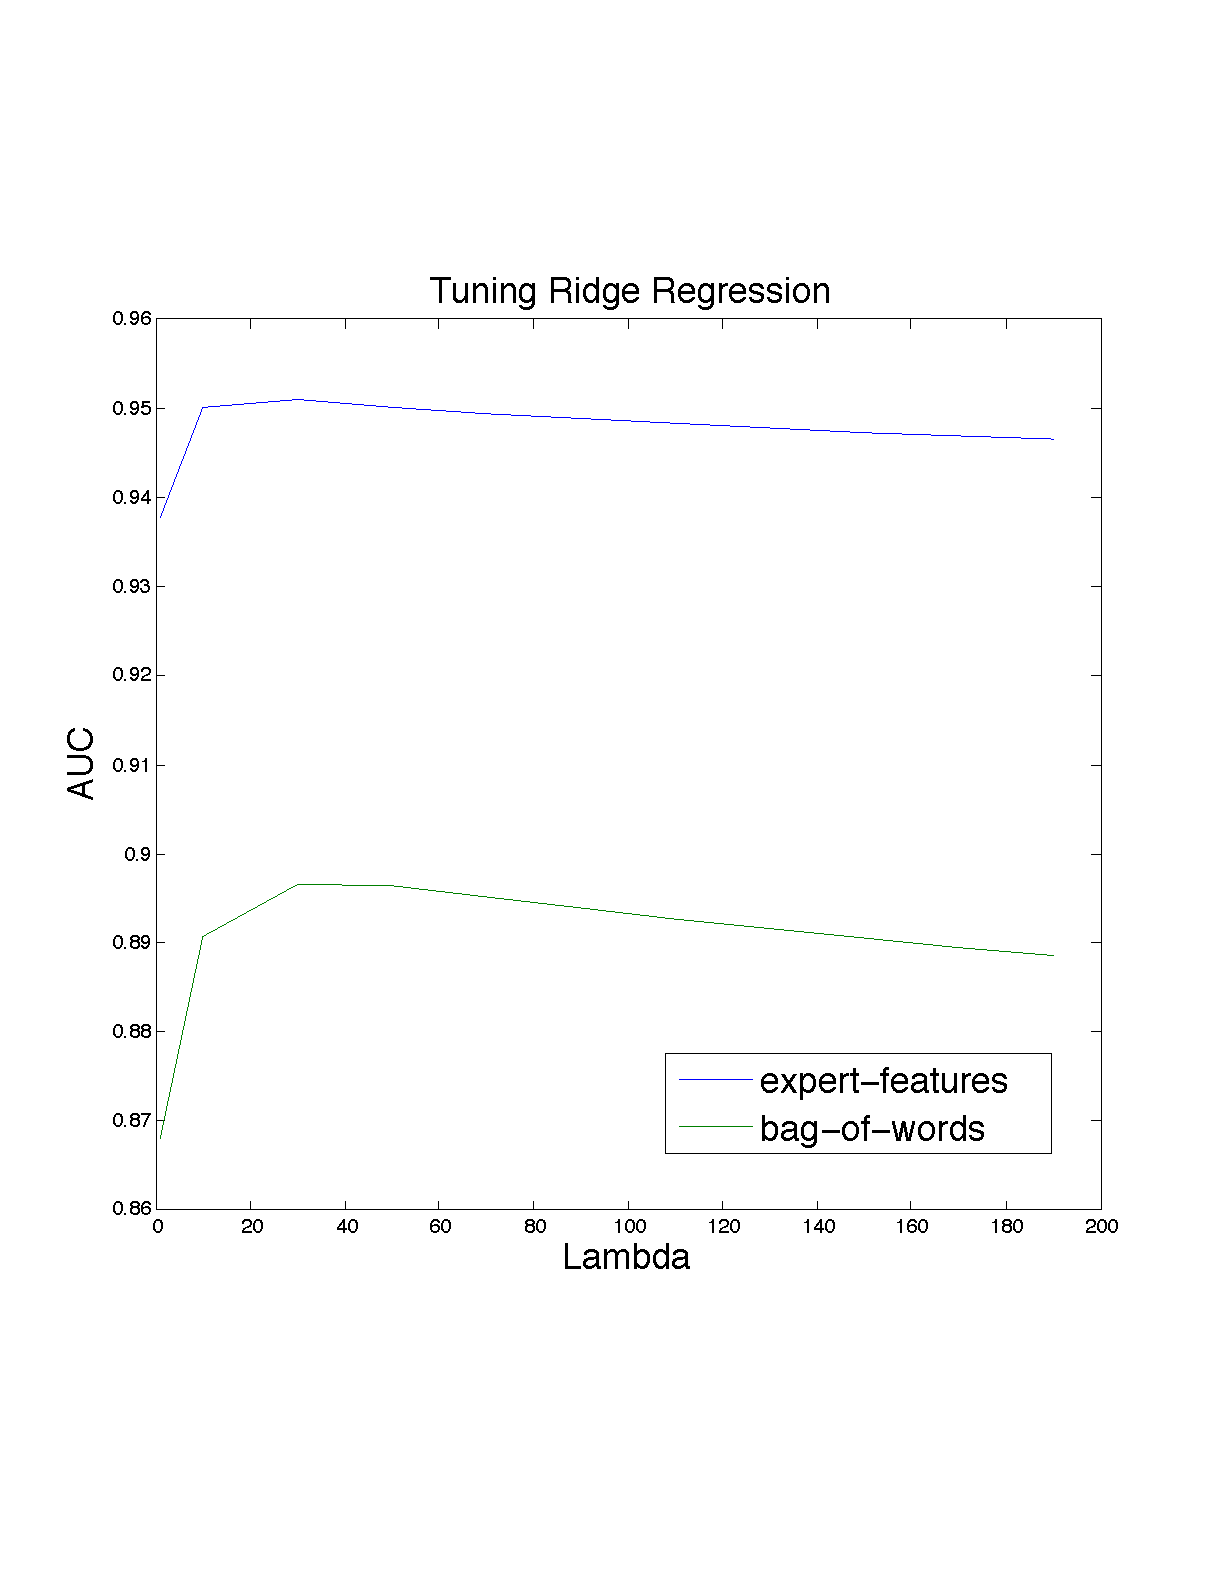
\includegraphics[width=\linewidth]{figures/linear-ridge.pdf}
    \caption{AUC based on varying lambda values for Ridge regression}
    \label{fig:lambda}
\end{figure}

\begin{figure}[h]
    \centering
    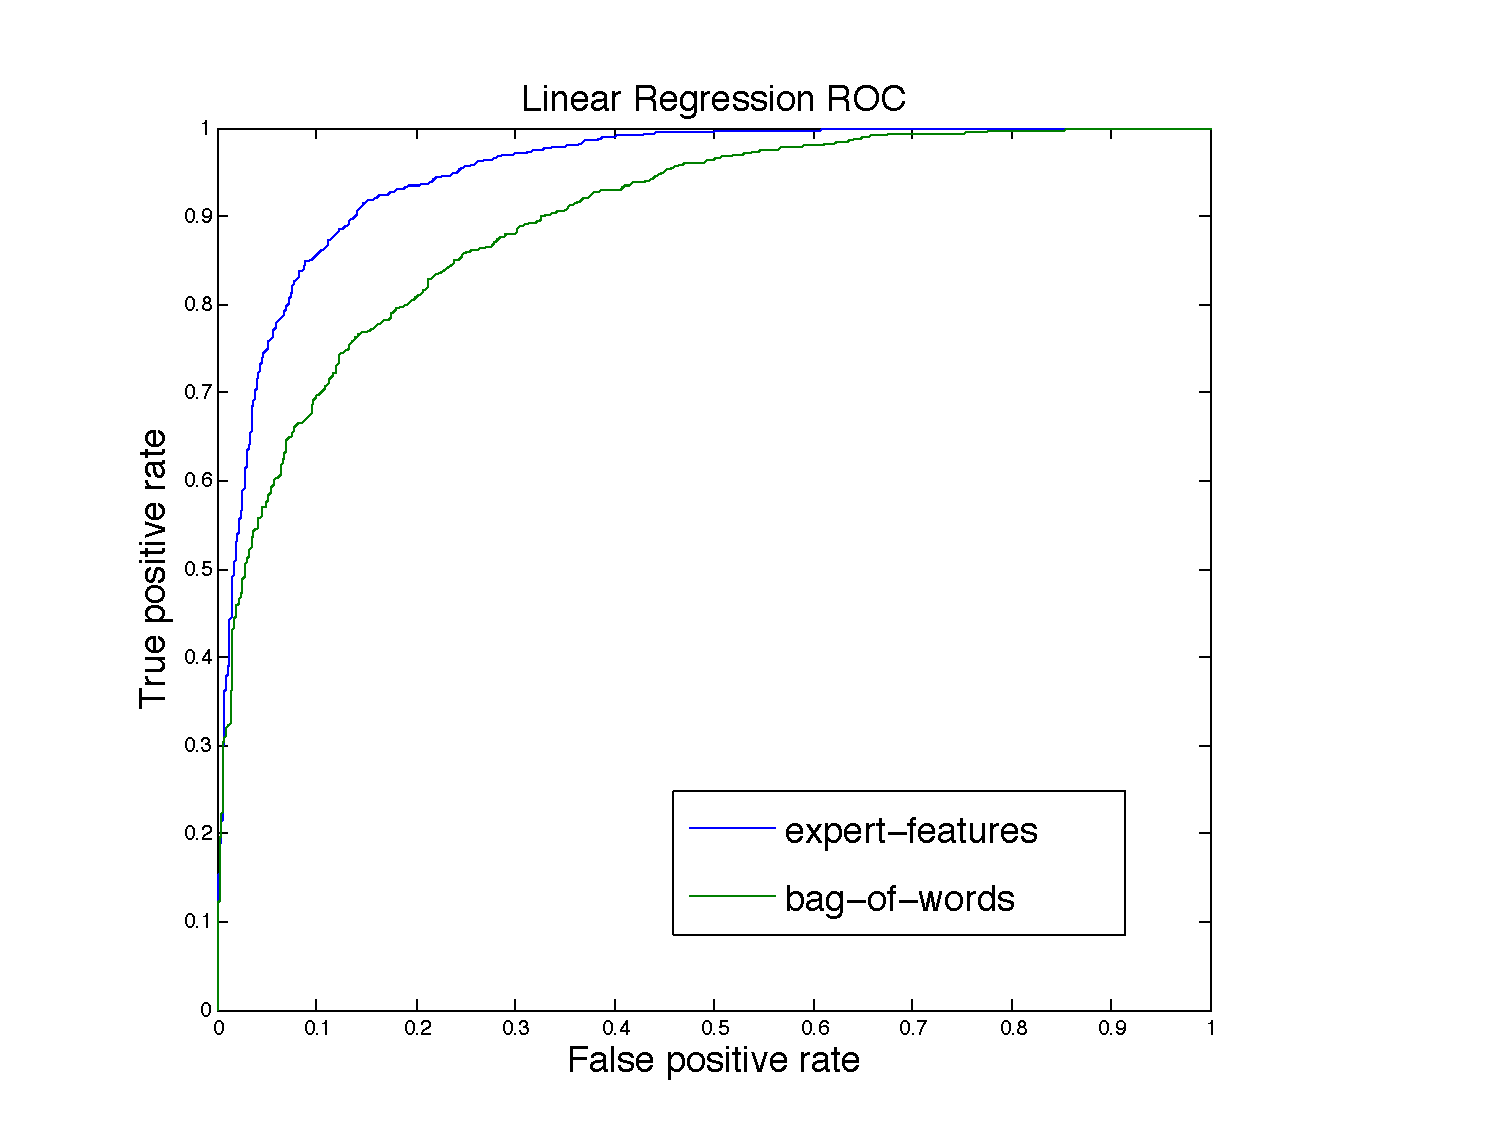
\includegraphics[width=\linewidth]{figures/linear-roc.pdf}
    \caption{Linear regression ROC curves for classifier using bag-of-words and bag-of-words with ``expert" features}
    \label{fig:roclin}
\end{figure}

Tables \ref{tab:lrfeats} and \ref{tab:lrfeatse} list the top-weighted terms for the bag-of-words and expert feature 
models. The spam-related words appear in line with our expectations, with sex-related terms prevalent, as well as
words that might indicate advertisements (``cafe4tune," for example, appears to be a competing SNS). Table \ref{tab:lrfeatse} 
shows that IP-profile country mismatch and membership of the IP-detected country in our ``high-risk" list were 
strong predictors that a message might be spam. Likewise, whether or not a user had photos was a righ-ranking indicator 
of ham.

% LR B-O-W
\begin{table}
\small
\begin{tabular}{l|l||l|l}
\multicolumn{2}{c}{\textbf{Ham}} & 
\multicolumn{2}{c}{\textbf{Spam}} \\
\hline
\textbf{Feature} & \textbf{Weight} & \textbf{Feature} & \textbf{Weight} \\
\hline
happy & -0.1314 & sex & 0.2295\\
hahaha & -0.13 & cafe4tune & 0.1906\\
turkey & -0.1271 & tony & 0.1715\\
learn & -0.124 & oky & 0.1549\\
fb & -0.1186 & photo & 0.1467\\
goin & -0.1177 & hehe & 0.1379\\
kk & -0.1164 & rochelle & 0.1346\\
uganda & -0.1159 & register & 0.1327\\
new & -0.1156 & irene & 0.1298\\
msn & -0.1114 & okay & 0.1294\\
ya & -0.11 & sexy & 0.1278\\
thx & -0.1095 & ali & 0.1199\\
question & -0.1095 & displaying & 0.1112\\
xxx & -0.1081 & ghana & 0.1110\\
joyce & -0.1078 & correctly & 0.1102\\
year & -0.1067 & ok & 0.1093\\
hw & -0.1067 & m? & 0.1087\\
snail & -0.1059 & sand & 0.1072\\
direct & -0.1052 & check & 0.1058\\
bonne & -0.1014 & sabina & 0.105\\
\end{tabular}
\caption{Linear regression top features (bag-of-words) with weights}
\label{tab:lrfeats}
\end{table}

% LR + expert
\begin{table}
\small
\begin{tabular}{l|r||l|r}
\multicolumn{2}{c}{\textbf{Ham}} & 
\multicolumn{2}{c}{\textbf{Spam}} \\
\hline
\textbf{Feature} & \textbf{Weight} & \textbf{Feature} & \textbf{Weight} \\
\hline
requests & -0.1349 & F-country\_match & 0.3365\\
giggle & -0.1257 & sex & 0.1954\\
turkey & -0.1213 & cafe4tune & 0.1723\\
hw & -0.1148 & register & 0.1324\\
F-photo\_exists & -0.1087 & F-spam\_country & 0.1231\\
xxx & -0.1047 & rochelle & 0.1054\\
goin & -0.1008 & m? & 0.1019\\
teacher & -0.1006 & tony & 0.1017\\
happy & -0.0912 & hehe & 0.0991\\
yie & -0.0904 & oky & 0.0968\\
tea & -0.089 & sexy & 0.0967\\
snail & -0.0852 & ewelina & 0.0874\\
malaysia & -0.084 & card & 0.0866\\
russian & -0.0832 & return & 0.0856\\
fall & -0.0805 & video & 0.0842\\
question & -0.0789 & pay & 0.0841\\
ann? & -0.0785 & nas? & 0.0839\\
learn & -0.0784 & model & 0.0826\\
new & -0.0783 & displaying & 0.0808\\
daichi & -0.0775 & k?  & 0.0806\\
\end{tabular}
\caption{Linear regression top features (bag-of-words \& expert features) with weights (Expert features
are denoted by an `F-' prefix)}
\label{tab:lrfeatse}
\end{table}

\subsection{Logistic Regression}

We attempted to train the multiple logistic regression classifier implemented by the ScalaNLP package, 
but encountered a bug that prevented the model from being generated correctly. With the expectation 
that SVMs would outperform logistic regression, we decided to focus our efforts on tuning the SVM 
instead of pursuing logistic regression. 

\subsection{Support Vector Machines (SVMs)}

%intro to svms

Support Vector Machines are a classification method that maps class examples (\eg messages) to points 
in space and aims to maximize the margin around a hyperplane separating the classes.\cite{boser}, \cite{cortesv95} 
Because the sets of points may not be linearly separable in the original dimension, a kernel trick can 
be used to fit the maximum-margin hyperplane in a higher-dimensional feature space (which may appear 
non-linear in the original input space).

We initially used ScalaNLP's built-in SVM solver, which implements the Pegasos maximization algorithm\cite{pegasos} 
as extended by Wang, Crammer and Vucetic\cite{wang2}. 
The optimizer runs stochastic subgradient descent on the primal objective 
using batches provided. However, the ScalaNLP SVM interface does not allow changing kernel functions or parameters, 
which seems to have led to the classifier's sub-par performance.

We then turned to LIBSVM, a library for SVM training and classification in C++ and Java, with wrappers for 
Python and other languages. The package allows one to specify the type of kernel to use, kernel parameters 
($\gamma$, $\rho$, $d$), as well as a soft margin parameter ($C$). We used Perl to convert the sparse feature 
matrices generated for use with ScalaNLP to a format recognized by LIBSVM. We then used one of the package's 
tools to perform simple scaling on the data. 

Given the complexity and time-intensive nature of choosing and testing parameters, the 
package includes a Python script that performs cross-validation to suggest appropriate 
$\gamma$ and $C$ values for the recommended Gaussian radial basis function (RBF) kernel. The RBF kernel is 
a real-valued function such that: 
$$K(\mathbf{x}_i, \mathbf{x}_j) = (\gamma\mathbf{x}_i^\intercal\mathbf{x}_j+r)^d, \gamma>0$$
We ran this script on a subset of 5000 messages with expert features to obtain $C = 8$ and $\gamma = 0.0078125$, 
which we used to tune the SVM we used to classify both the bag-of-words and expert feature models.

\subsection{SVM Results}

Our initial results using the Pegasos SVM solver included in ScalaNLP were lower than expected. The 
classifier trained on the bag-of-words feature set (from 22k messages) yielded a 77\% mean accuracy 
over 10-fold cross-validation. The addition of expert features actually decreased this accuracy to 
51\%. 

Table \ref{tab:svmfeats} provides a list of top features for the bag-of-words and expert 
feature models. We see that for the bag-of-words classifier, the words ``year," ``new," ``happy,"  
``2012," ``wish," and ``you" all have high weights, which makes sense given that the ham data was 
collected around the beginning of 2012. The lists include a number of stop words, such as ``ok," 
``me" and ``it," which should ideally not be highly weighted. While we did not remove stop words for this 
project, this is something that we could consider doing in the future. 

The table of top terms reveals that three expert features: account lifetime, friends and 
recipient age, are weighted very heavily in comparison to the remaining features. These 
skewed weights (and the inability to tune the SVM solver via ScalaNLP) prompted us to test LIBSVM 
on the same data.

\begin{table}
\small
\begin{tabular}{l|r||l|r}
\multicolumn{2}{c}{\textbf{Bag-of-Words}} & 
\multicolumn{2}{c}{\textbf{Expert Features}} \\
\hline
\textbf{Feature} & \textbf{Ham Wt.} & \textbf{Feature} & \textbf{Ham Wt.} \\
\hline

year & 0.2253 & F-account\_lifetime & -0.9800\\
new & 0.2250 & F-friends & -0.3671\\
am & -0.1722 & F-recip\_age & -0.2129\\
happy & 0.1600 & F-age & -0.1830\\
d & 0.1513 & i & -0.05231\\
ok & -0.1497 & you & -0.0483\\
yahoo & -0.1360 & to & -0.04026\\
it & 0.1200 & and & -0.03636\\
me & -0.1180 & F-month\_of\_birth & -0.03452\\
too & 0.1173 & F-country\_match & -0.0269\\
i'm & 0.1116 & me & -0.0224\\
haha & 0.0998 & am & -0.0220\\
can & -0.0971 & my & -0.0209\\
okay & -0.0947 & ? & 0.0199\\
dear & -0.0882 & ? & 0.0191\\
p & 0.0862 & a & -0.01573\\
here & -0.0844 & your & -0.01554\\
2012 & 0.084 & F-photo\_exists & -0.0146\\
wish & 0.0836 & the & -0.01412\\
doing & -0.0779 & F-sex & -0.01258\\

\end{tabular}
\caption{SVM term weights (ScalaNLP Pegasos implementation). The spam term weights were the same, but opposite signs.
Question marks indicate strings in a different character encoding.}
\label{tab:svmfeats}
\end{table}

Our results with LIBSVM's RBF kernel were consistently better than any of the other classifiers we tested. We 
evaluated the classifier's performance on five pairs of bag-of-words and expert feature data sets ranging in 
size from 2000 to 100k messages. Table \ref{tab:svmacc} shows results of 10-fold cross-validation. Our mean 
accuracy over the bag-of-words data sets was 85.73\% and 98.41\% over the bag-of-words with expert features. We 
observed a slight decrease in performance on the bag-of-words data sets as the data size grew. Figure \ref{fig:roc-25}
shows the AUCs and ROC curves for the 50k data sets, making clear the the significantly greater AUC resulting 
from the addition of expert features. As expected, however, both the ScalaNLP and LIBSVM implementations 
took substantially longer to train than NB and LR.

\begin{table}
\small
\begin{tabular}{r|r|r}
\hline
\textbf{Dataset Size} & \textbf{Bag-of-Words} & \textbf{Expert Features} \\
\hline
2000 & 86.70\% & 98.35\% \\
10000 & 86.23\% & 98.49\% \\
22000 & 86.81\% & 98.33\% \\
50000 & 84.59\% & 98.43\% \\
100000 & 84.33\% & 98.45\% \\
\end{tabular}
\caption{SVM 10-fold cross-validation accuracy over data sets of varying sizes (half spam, half ham)} 
\label{tab:svmacc}
\end{table}

\begin{figure}[h]
    \centering
    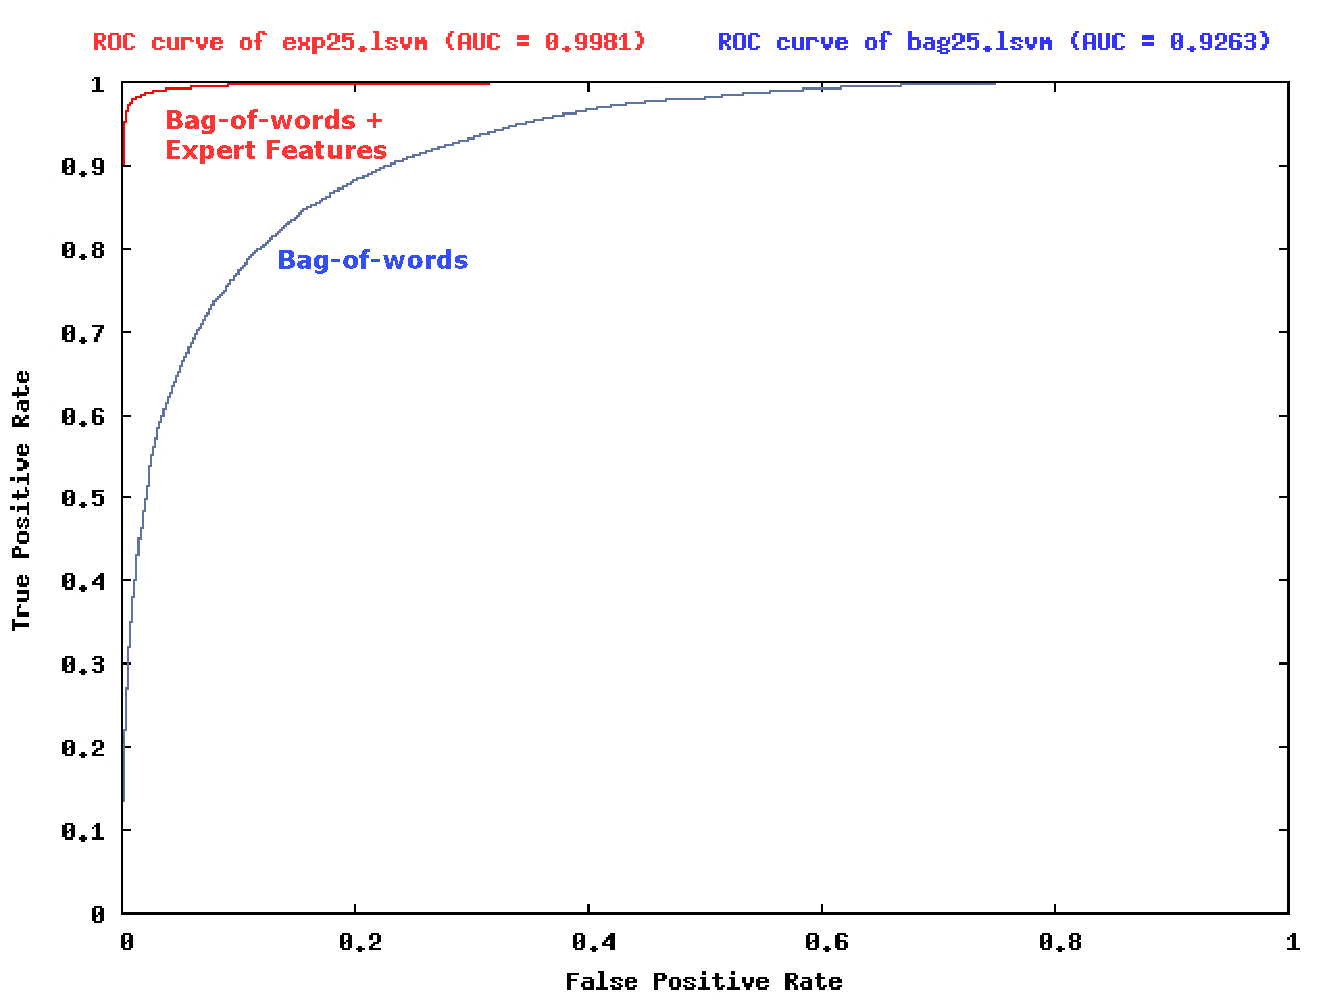
\includegraphics[width=\linewidth]{figures/roc-25.pdf}
    \caption{LIBSVM ROC curves for classifier using bag-of-words and bag-of-words with ``expert" features on 50k messages 
     (25k spam, 25k ham)}
    \label{fig:roc-25}
\end{figure}

\section{Future Work}

\subsection{Data Collection}

The ham message collection methodology used in this project may have been flawed, leading to questionable 
performance for several classifiers. The 2 million ham messages were sent over a span of 10 days, from 
December 23, 2011 to January 1, 2012. While we chose the corpus' start date as exactly four months before 
extracting the data, the coincidental timing with a global holiday seems to have introduced unusual 
skew in the bag-of-words features. In contrast, the majority of messages in the spam corpus span a period of 
7 months, with only a slight linear increase in volume over the interval.  Consequently, as seen in 
the linear regression and SVM feature weight tables, words typically associated with the New Year gained 
undue weight during classification.  We plan to address this issue by creating a new ham message corpus 
through sampling that matches the temporal distribution of spam messages more closely.

Another direction for future research would be to examine data other than messages. We have access to millions 
of wall posts and photo comments, making it possible to investigate the characteristics of spam in these genres. 
Wall posts and comments tend to be comparatively short, which should present a slightly different classification 
problem.

We have also recently observed spammers attacking the report system by reporting large numbers of legitimate users 
with complaints consisting of nonsensical text or form messages. In addition to offering another application for 
classifiers, the data we are collecting should offer a window into the retaliatory techniques of miscreants on 
SNSs.

\subsection{Spam Grouping}

As a part of this project, we performed some qualitative analysis on spam and differentiated between 
some major categories of undesirable messages that we observed on the InterPals web site. However, we would 
like to gain a better understanding of the relative volume of each type of scam. To this end, we plan to 
experiment with clustering algorithms to attempt to identify and quantify subclasses of spam. 

Furthermore, characteristics of spam messages vary substantially depending on the type of spam or scam in question. 
The classifiers that we trained and evaluated in this project all spam messages as a single category. We are currently 
investigating multiclass classifiers as a potential tool to identify the type of 
spam in question with greater precision. Specifically, we are considering multiclass SVMs, which reduce 
multiclass problems into multiple binary classification problems.\cite{duan} 

From a site's perspective, this finer granularity is desirable not only 
because specialty classifiers could be trained to recognize specific classes of spam, but also in order to 
trigger different courses of action (\eg automatic account deletion, warning messages, reports to human moderators) 
based on the class and probability of spam detected.

We are currently extending the moderation interface to include more specific tagging capabilities, which should aid 
in generating labels for multiclass classifiers and for seeding semi-supervised clustering algorithms (see Basu et al. 
\cite{basu}).

\subsection{Features}

In this project, we chose only a small subset of ``expert" features to use. However, we believe that 
it would be beneficial to train and evaluate the classifiers on a wider range of features. The features 
would include both the ones we extracted in this project but omitted from the classifier features matrices, 
as well as new features. Adding N-grams and message similarity tests seem particularly promising. 
N-grams would allow the classifier to take into account certain phrases \eg{``Western Union" or ``money transfer"}. 

We have also recently begun to collect browser fingerprints from users based on user agent 
and JavaScript-acquired browser plugin details, time zone, screen size, color depth, system fonts, 
keyboard layout and locale information. Subsequent classifiers could leverage this information either 
as a hash that effectively tags individual known spammers or in part, adding features based on 
time zone or keyboard layout.

It is also anecdotally clear from moderator log messages that spammers re-use their profile photos and 
these photos are often of celebrities or simply stock photos. Fingerprinting and perceptual hash techniques 
such as Marr wavelet, discrete cosine transform (DCT), color histograms, etc., which provided by the 
pHash library\cite{phash}, seem to promising in detecting image re-use. 

Server access logs, search logs and user viewing histories from InterPals, all of which 
are available to us, offer another avenue for future research. It is conceivable that certain 
spammers may have similar site usage patterns, in terms of HTTP request intervals, search queries, 
and so on, which might prove useful in their detection.

\subsection{Site Implementation}

Given the promising results of SVM classifiers in this project, we plan to test and implement a classifier that will 
be integrated into the site application code itself. Initially, we envision this as a system that automatically flags 
potential spam messages and brings them to the attention of human moderators. Moderators will then be able to manually 
make a decision as to whether the messages are spam or not. In order to diminish the effect of subjectivity or moderator 
error, each message will be vetted by several moderators, and the majority decision will be accepted as ground ``truth." 
Recording these messages and moderator decision will allow us to further evaluate the performance of these classifiers in 
the ``wild."

\section{Conclusion}

In this paper, we presented a brief overview of the breakdown of spam and scams on the InterPals web site. 
We then examined a number of statistics on both public and private data that showed that spam users, even when 
grouped together without regard to their specific angle of attack, share a number of characteristics that differentiate 
them from legitimate users. We trained and evaluated Naive Bayes, linear regression and SVM classifiers on a subset 
of the 4 million messages on which we collected feature statistics. Our evaluation compared the performance of 
each classifier on bag-of-word representations of message text vis-\`{a}-vis the combination of bag-of-word features 
with a number of ``expert features." We found that SVMs using an RBF kernel on LIBSVM outperformed the other 
classifiers. In both the linear regression and SVM cases, the addition of expert features substantially increased 
the classifier's accuracy, underscoring the impact of supplementary account-related features in detecting spam on 
SNSs.

\bibliographystyle{abbrv}
\bibliography{paper}

\balancecolumns
\end{document}
